\documentclass{beamer}
\usepackage[utf8]{inputenc}

\usetheme{Madrid}
\usecolortheme{default}
\usepackage{amsmath,amssymb,amsfonts,amsthm}
\usepackage{txfonts}
\usepackage{tkz-euclide}
\usepackage{listings}
\usepackage{adjustbox}
\usepackage{array}
\usepackage{tabularx}
\usepackage{gvv}
\usepackage{lmodern}
\usepackage{circuitikz}
\usepackage{tikz}
\usepackage{graphicx}

\setbeamertemplate{page number in head/foot}[totalframenumber]

\usepackage{tcolorbox}
\tcbuselibrary{minted,breakable,xparse,skins}



\definecolor{bg}{gray}{0.95}
\DeclareTCBListing{mintedbox}{O{}m!O{}}{%
	breakable=true,
	listing engine=minted,
	listing only,
	minted language=#2,
	minted style=default,
	minted options={%
		linenos,
		gobble=0,
		breaklines=true,
		breakafter=,,
		fontsize=\small,
		numbersep=8pt,
		#1},
	boxsep=0pt,
	left skip=0pt,
	right skip=0pt,
	left=25pt,
	right=0pt,
	top=3pt,
	bottom=3pt,
	arc=5pt,
	leftrule=0pt,
	rightrule=0pt,
	bottomrule=2pt,
	toprule=2pt,
	colback=bg,
	colframe=orange!70,
	enhanced,
	overlay={%
		\begin{tcbclipinterior}
			\fill[orange!20!white] (frame.south west) rectangle ([xshift=20pt]frame.north west);
	\end{tcbclipinterior}},
	#3,
}
\lstset{
	language=C,
	basicstyle=\ttfamily\small,
	keywordstyle=\color{blue},
	stringstyle=\color{orange},
	commentstyle=\color{green!60!black},
	numbers=left,
	numberstyle=\tiny\color{gray},
	breaklines=true,
	showstringspaces=false,
}
\begin{document}

\title 
{12.54}
\date{5 Oct,2025}

\author 
{Naman Kumar-EE25BTECH11041}
\graphicspath{./figs}


\frame{\titlepage}
\begin{frame}{Question)}
For a matrix
\begin{align}
    \vec{M}=\begin{pmatrix}
        \frac{4}{5} & -\frac{3}{5} \\\frac{3}{5} & x
    \end{pmatrix}
\end{align}
the transpose of the matrix is equal to the inverse of the matrix, i.e., $\vec{M}^T=\vec{M}^{-1}$.The value of x is given by
\end{frame}
\begin{frame}{Solution}
\begin{align}
    \vec{M}^T=\vec{M}^{-1} \label{1}
\end{align}
Multiple $\eqref{1}$ with $\vec{M}$
\begin{align}
    \vec{M}\vec{M}^T=\vec{I}
\end{align}
\end{frame}
\begin{frame}{Solution}
$\vec{M}$  is orthogonal matrix
\begin{align}
\begin{pmatrix}\frac{4}{5} & \frac{-3}{5} \\ \frac{3}{5} & x\end{pmatrix}\begin{pmatrix}\frac{4}{5} & \frac{-3}{5} \\ \frac{3}{5} & x\end{pmatrix}^T=\begin{pmatrix}1&0\\0&1\end{pmatrix}\\
\begin{pmatrix}\frac{16}{25}+ \frac{9}{25} & \frac{-12}{25}+\frac{3x}{25} \\
\frac{-12}{25} +\frac{3x}{25} & \frac{9}{25}+x^2\end{pmatrix}=\begin{pmatrix}1&0\\0&1\end{pmatrix}
\end{align}
\end{frame}
\begin{frame}{Solution}
\begin{align}
\frac{-12}{25}+\frac{3x}{25}=0\\
x=\frac{4}{5} \label{2} \\ 
\frac{9}{25}+x^2=1\\
x^2=\frac{16}{25}\\
x=\pm \frac{4}{5} \label{3}
\end{align}
\end{frame}
\begin{frame}{Solution}
from $\eqref{2}$ and $\eqref{3}$
\begin{align}
    x=\frac{4}{5}
\end{align}
\end{frame}

\begin{frame}{Figure}
    \begin{figure}[H]
    \centering
    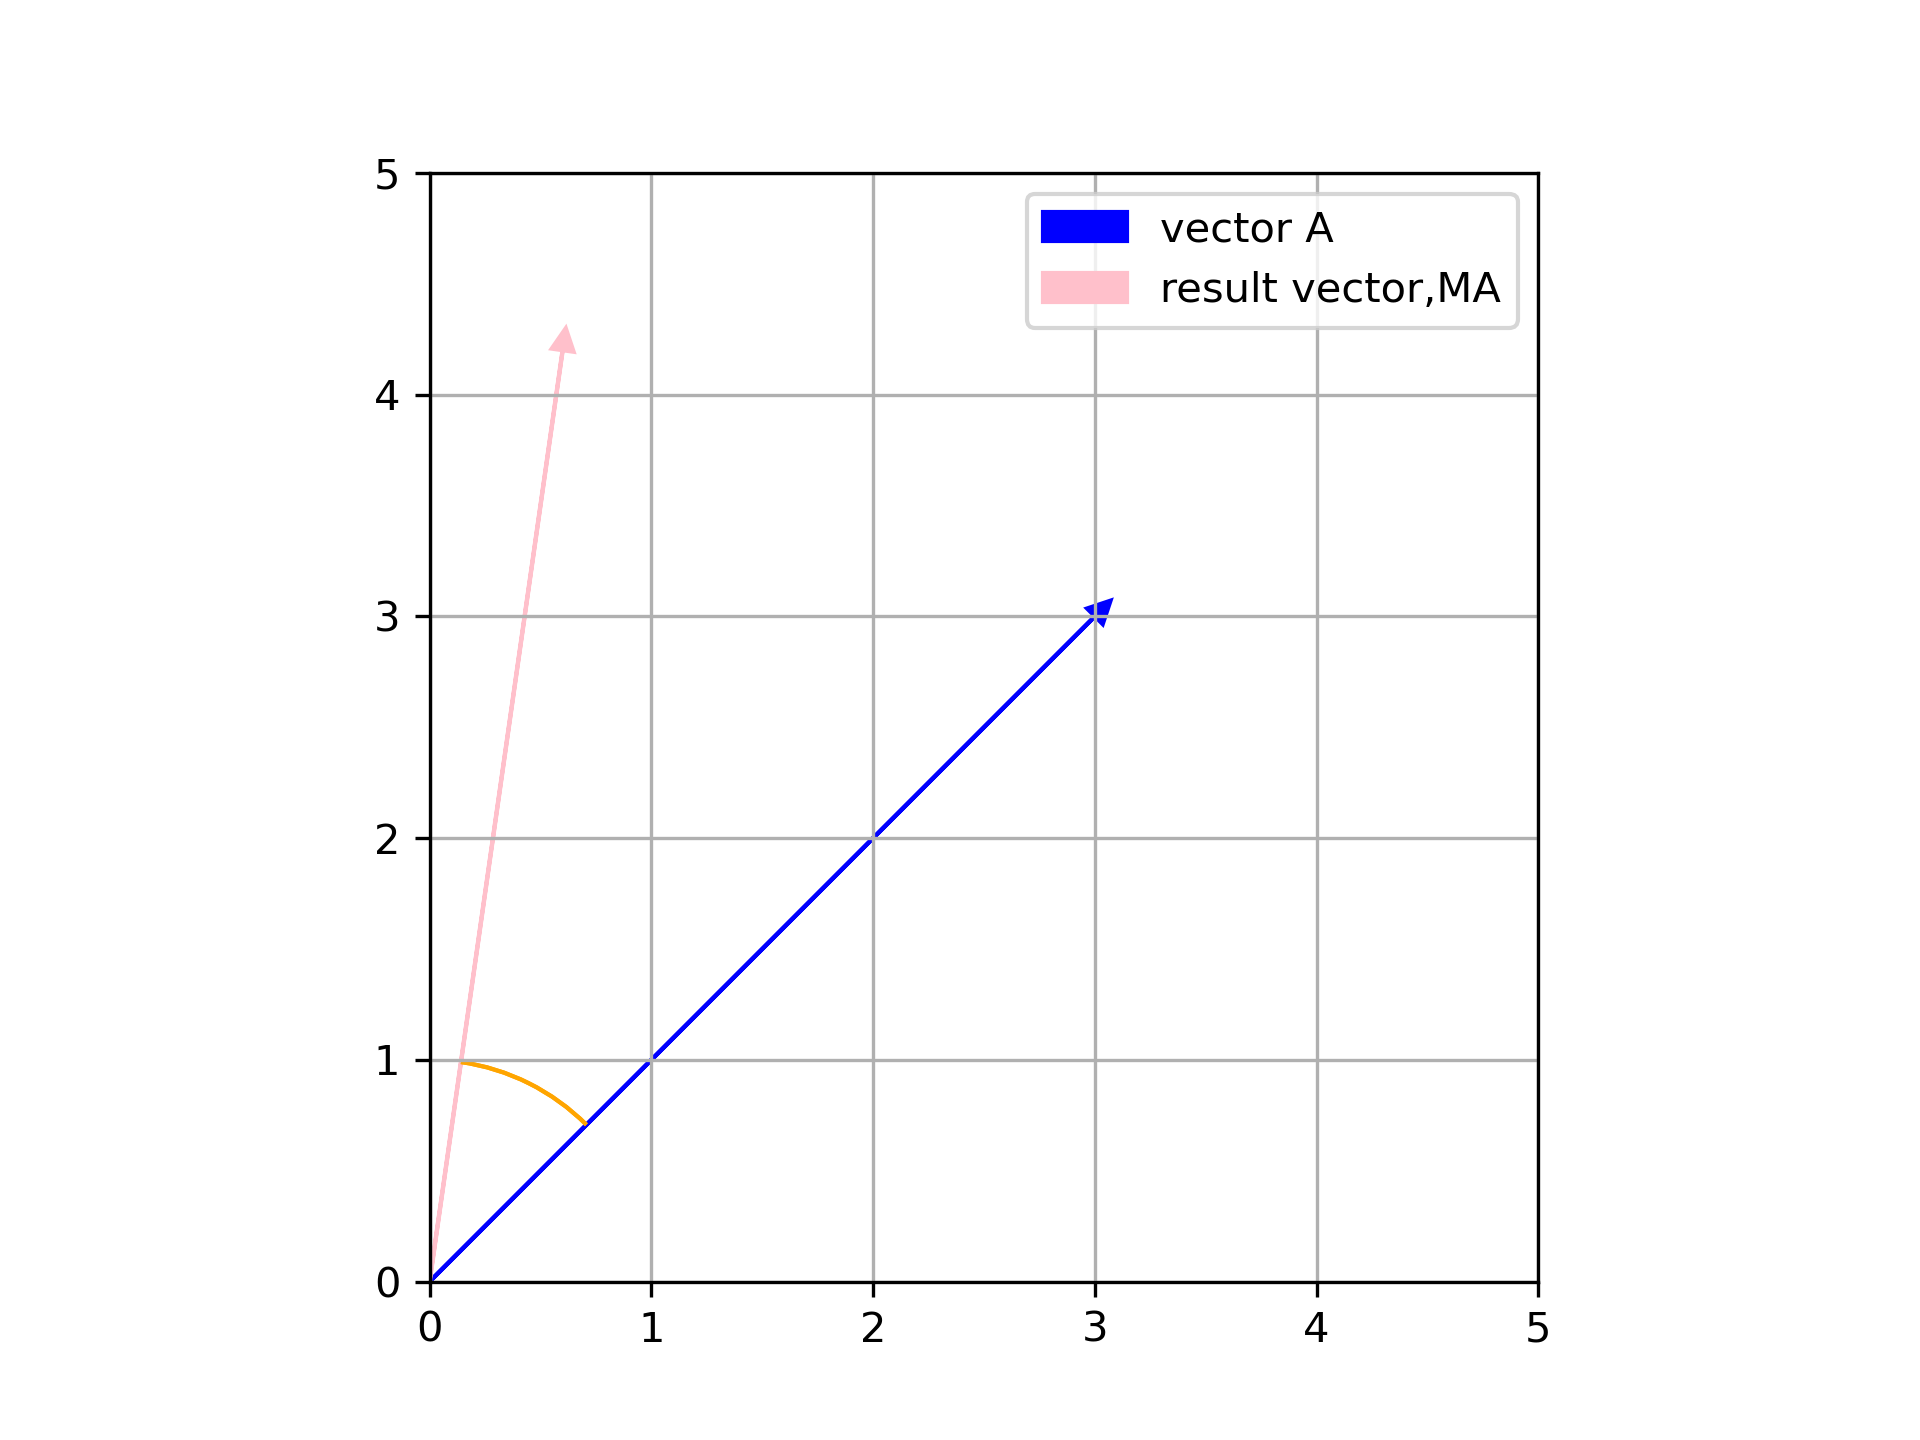
\includegraphics[width=0.7\columnwidth]{figs/fig1.png}
    \caption{1}
    \label{fig:placeholder}
\end{figure}
\end{frame}
\begin{frame}{Figure}
\begin{figure}[H]
    \centering
    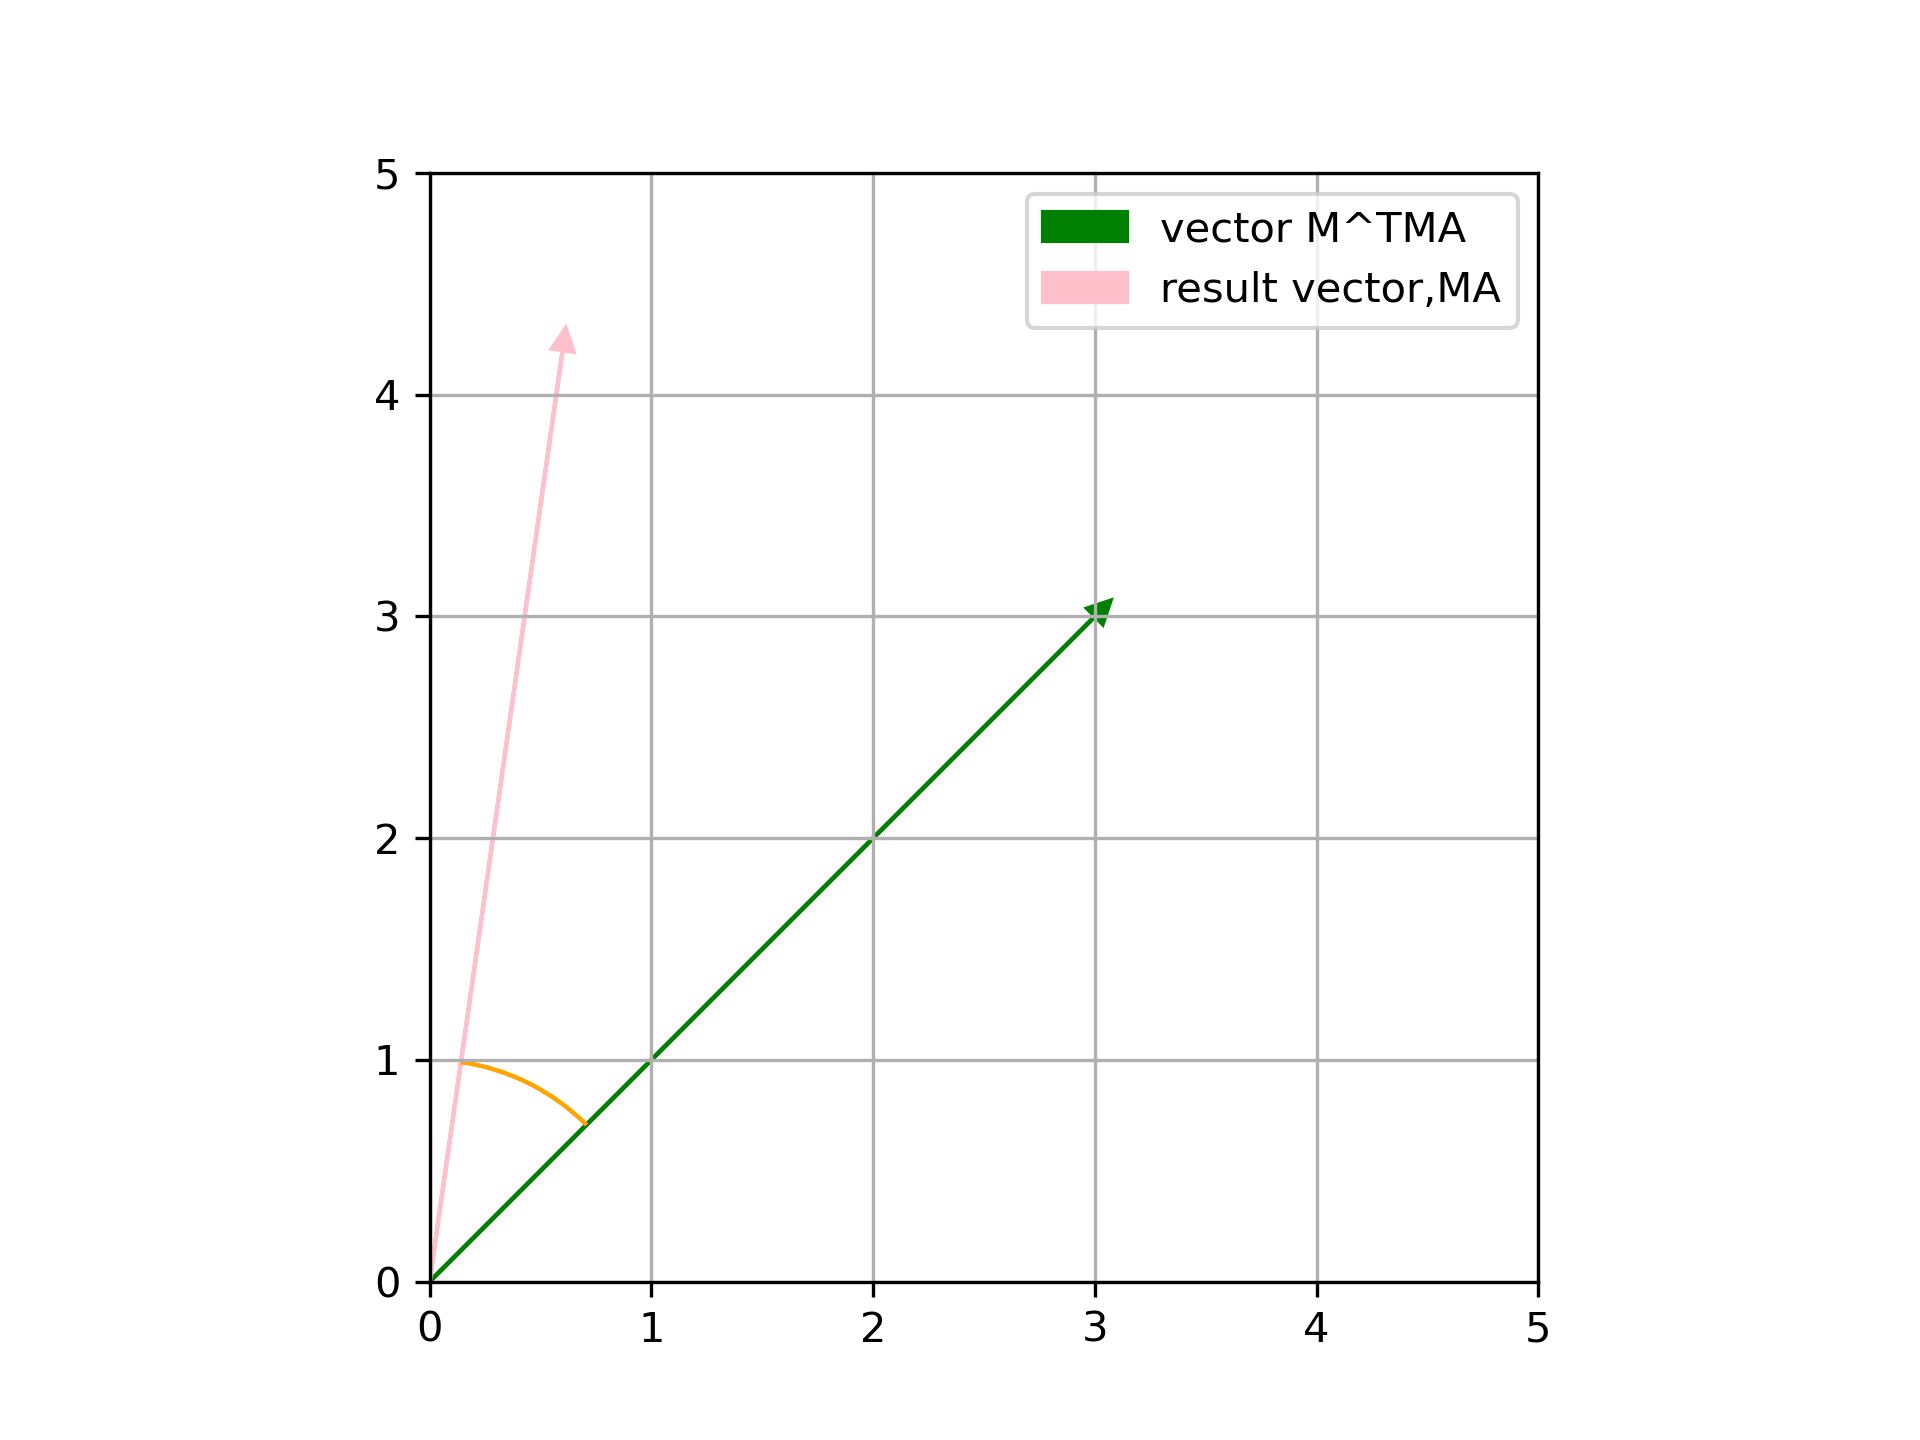
\includegraphics[width=0.7\columnwidth]{figs/fig2.png}
    \caption{2}
    \label{fig:placeholder}
\end{figure}
\end{frame}
\begin{frame}[fragile]
\frametitle{Direct Python 1}
\begin{lstlisting}
import numpy as np
import matplotlib.pyplot as plt
from matplotlib.patches import Arc


x = np.array([3 ,3]).reshape(-1,1)
y= np.array([3,1])
m = np.array([[0.8,-0.6],[0.6,0.8]])
fig, ax = plt.subplots()

ax.arrow(0, 0, 3, 3, head_width=0.1, head_length=0.1, fc='blue', ec='blue', label="vector A")
c = m@x
ax.arrow(0, 0, c[0,0], c[1,0], head_width=0.1, head_length=0.1, fc='pink', ec='pink',label="result vector,MA")
\end{lstlisting}
\end{frame}
\begin{frame}[fragile]
\frametitle{Direct Python 1}
\begin{lstlisting}
center = (0, 0)
radius = 1.0
start_angle = 45
end_angle = 81.87

arc = Arc(center, 2 * radius, 2 * radius, theta1=start_angle, theta2=end_angle, 
          edgecolor='orange', linewidth=1)

ax.add_patch(arc)
ax.add_patch(arc)
\end{lstlisting}
\end{frame}
\begin{frame}[fragile]
\frametitle{Direct Python 1}
\begin{lstlisting}
ax.set_aspect('equal', adjustable='box')
ax.set_xlim(0, 5)
ax.set_ylim(0, 5)
plt.legend()
plt.grid()
plt.savefig("fig1.png", dpi=300)
plt.show()

\end{lstlisting}
\end{frame}
\begin{frame}[fragile]
\frametitle{Direct Python 2}
\begin{lstlisting}
import numpy as np
import matplotlib.pyplot as plt
from matplotlib.patches import Arc


x = np.array([3 ,3]).reshape(-1,1)
y= np.array([3,1])
m = np.array([[0.8,-0.6],[0.6,0.8]])
fig, ax = plt.subplots()
\end{lstlisting}
\end{frame}
\begin{frame}[fragile]
\frametitle{Direct Python 2} 
\begin{lstlisting}
ax.arrow(0, 0, 3, 3, head_width=0.1, head_length=0.1, fc='green', ec='green', label="vector M^TMA")
c = m@x
ax.arrow(0, 0, c[0,0], c[1,0], head_width=0.1, head_length=0.1, fc='pink', ec='pink',label="result vector,MA")
center = (0, 0)
radius = 1.0
start_angle = 45
end_angle = 81.87
\end{lstlisting}
\end{frame}
\begin{frame}[fragile]
\frametitle{Direct Python 2} 
\begin{lstlisting}
arc = Arc(center, 2 * radius, 2 * radius, theta1=start_angle, theta2=end_angle, 
          edgecolor='orange', linewidth=1)

ax.add_patch(arc)
ax.add_patch(arc)

ax.set_aspect('equal', adjustable='box')
ax.set_xlim(0, 5)
ax.set_ylim(0, 5)
plt.legend()
plt.grid()
plt.savefig("fig2.png", dpi=300)
plt.show()

\end{lstlisting}
\end{frame}
\end{document}